\documentclass[12pt]{article}

% Packages
\usepackage{graphicx}
\usepackage{subcaption}
\usepackage{hyperref}
\usepackage{gensymb}
\usepackage{scrextend}
\usepackage{tcolorbox}
\usepackage{amsmath}
\usepackage{rotating}
\usepackage{makecell}
\usepackage{capt-of}
\usepackage{hyperref}

\usepackage[margin=1in]{geometry}

\graphicspath{{./graphics/}}

\usepackage[utf8]{inputenc}

\setlength{\parindent}{0pt}

% Custom commands
\newcommand{\cotwo}{CO\textsubscript{2} }

\title{Smart Energy HS18 Summary}
\author{Joel Oskarsson (\texttt{ojoel@student.ethz.ch})
\\
\\
For more information see: \href{https://github.com/joelnir/SmartEnergy/}{\texttt{github}}
}

\begin{document}
\maketitle

\tableofcontents
\newpage

\section{Energy and Electricity}
There is a mismatch between what many people believe uses most energy and reality.\\
Energy usage commonly\\
\textbf{overestimated}: warmwater, electronic equipment\\
\textbf{underestimated}: heating, personal car\\

\subsubsection{Energy in the industrial age}
Energy has been the fuel of the industrial age.
It has been a cheap driver of economic growth.
Measuring \cotwo in the atmosphere throughout hundreds of years we can see a big increase around 1800, likely caused by the invention of the steam engine. This development has continued and energy has become a major problem of the \textbf{late} industrial age.\\

\textbf{Energy problems}
\begin{itemize}
    \item Environmental issues (\cotwo etc.)
    \item Cost of acqusition
    \item Dependence on other countries (geopolitics)
    \item Renewable resources come with their own problems (unreliable, undispatchable)
\end{itemize}

\subsection{Energy}
Electricity $\subset$ Energy\\

Often energy usage leads to \cotwo emissions, which is one of the main modern day problems concerning energy.\\

The physical unit of energy is Joule. 1 J $=$ 1 Ws, the work required to produce one W of power for one second.
The sun yearly outputs $\sim 10^{13}$ ZJ.
Human society only need a tiny fraction of this energy which leads to a big engineering problem.
The world yearly energy consumption is $\sim 0.627$ ZJ, which corresponds to $\sim 2000$ J / person at any instant.
This number is higher in highly developed countries (Europe etc.).\\

What can we do with \textbf{1 Joule}
\begin{itemize}
    \item Lift an apple 1 meter
    \item Send $\sim$ 1 MB over WiFi
    \item Make a 2 second phonecall
    \item Drive a car 0.35 mm
\end{itemize}

Key idea of smart energy technology is that communication uses much less energy than transportation and heating.
We can save energy in these areas by using more ICT.

\subsubsection{Primary and Final Energy}
Total energy \textbf{consumption} (supply) is different than actual \textbf{end usage} due to energy loss.
Consider for example transforming coal into electricity.
In this process 60\% of the energy is lost.
This motivates a concept of \textbf{quality} of energy.
Heat is low-quality energy, electricity is high-quality energy.\\

Final energy can be seen as energy used on site, for example in a home.
In final energy electricity usage is comparable to other sources, but because electricity generation often require multiple units of lower quality sources it has a larger footprint in the primary energy consumption.\\

\begin{figure}
    \centering
    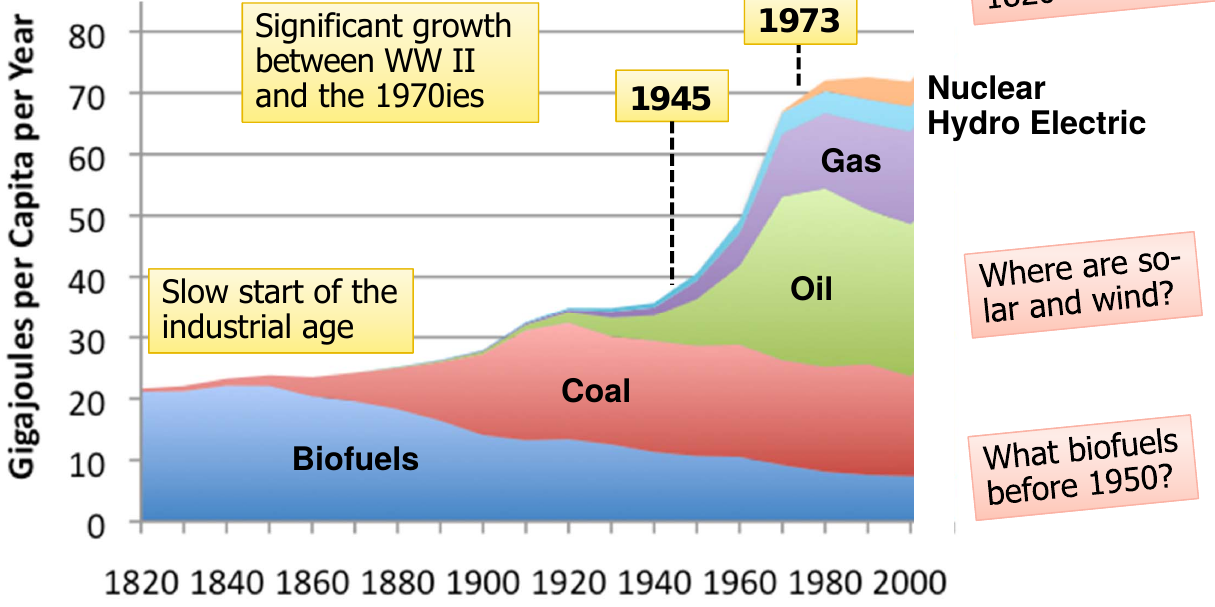
\includegraphics[width=0.7\linewidth]{primary_energy_consumption}
    \caption{Primary Energy Consumption per Capita}
    \label{fig:primary_energy}
\end{figure}

In figure \ref{fig:primary_energy} we can see trends in primary energy.
Note the decrease of biofuels, the rise and fall of oil, the increased usage of gas and the missing solar and wind power. It is clear that the total primary energy consumption has grown, but flattened out since 1973.\\

Since the 70s the primary energy consumption per capita in the US and Europe has stayed mostly the same.
Since 2000 we do however see a large increase in Asia and Africa.
This combined with a large population increase in these areas predict a future energy challenge.\\

There is a clear correlation between GDP (Gross Domestic Product) and primary energy consumption per capita. The increase of GDP in Asia and Africa also points towards a future energy consumption increase.

\subsubsection{Energy usage by types}
In 2016 only $\sim$ 9\% of energy used was estimated to come from renewable resources.
Less than 2\% of this was from so called new renewables (solar PV, wind etc.).
Changes in what types of resources is used is very slow due to long asset lifetimes.\\

\begin{figure}
    \centering
    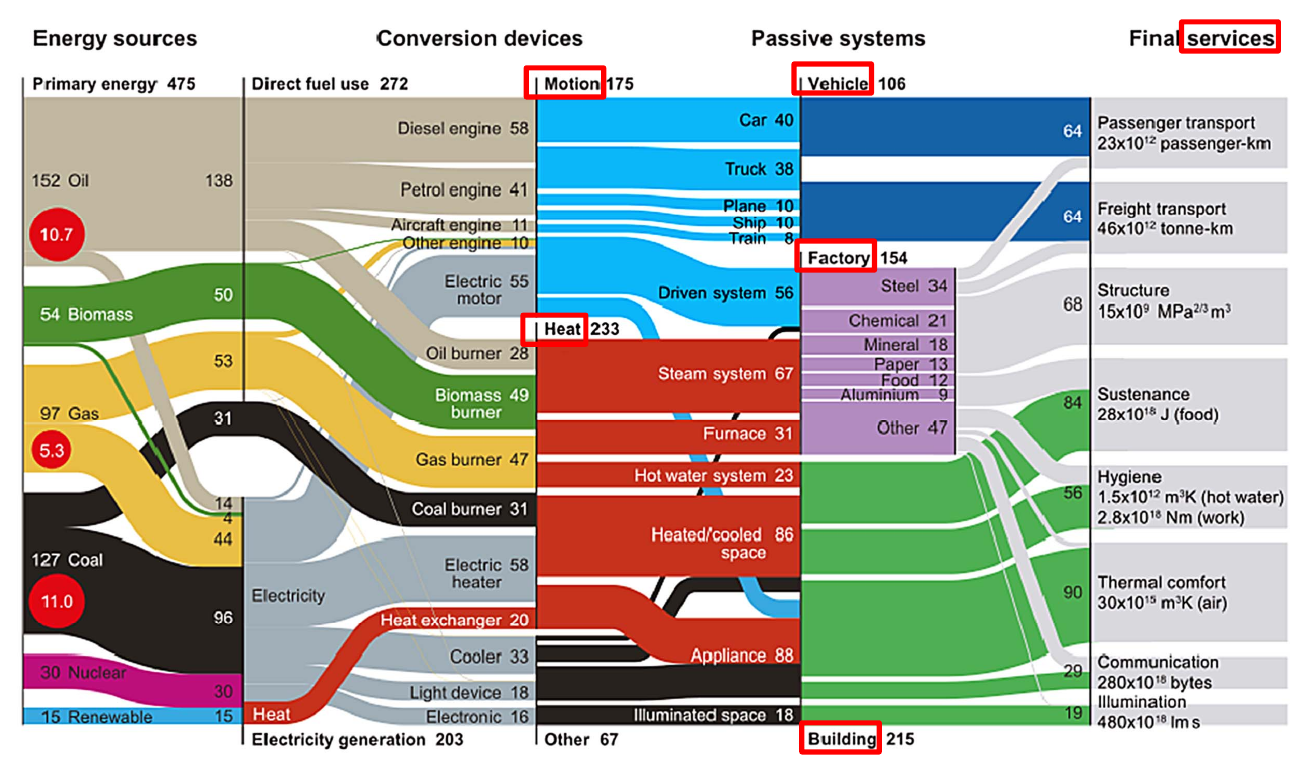
\includegraphics[width=\linewidth]{sankey_world}
    \caption{World energy flow 2005}
    \label{fig:sankey_world}
\end{figure}

Sankey diagrams visualize how energy transfers between processes.
They start in types of primary energy and ends in energy used in different sectors.
A sankey diagram for world energy flow 2005 can be seen in figure \ref{fig:sankey_world}.\\

In Switzerland the use of oil increased drastically up until the oil crisis in 1973.
Ater that the oil use has decreased and use of electricity and natural gas increased.

\subsubsection{Oil Crisis}
The 1973 oil crisis was a consequence of an oil embargo from Arab Petroleum Exporting Countries.
The reason for the embargo was related to US support of Israel.
During the oil crisis prizes for gasoline rose and rations were proclaimed in many countries. The crisis ended with the embargo in 1974, but the event impacted the future use of oil.

\subsubsection{Swiss Nuclear Phase Out}
Switzerland is currently committed to phasing out nuclear power.
This represents a big challenge since about 40\% of Swiss power comes from nuclear.
There are little opportunity to increase hydro power, so one discussed approach is to use more natural gas.
This is however controversial since it would carbonize Swiss electricity.

\subsection{Electricity Production}

\subsubsection{Swiss Hydro Energy}
Hydropower represents more than half of Swiss electricty production and will take up an even larger fraction as nuclear is phased out.
The electricity production from hydro has mostly stayed constant in the past 40 years.
Other renewables represent a very small fraction ($<$ 5\% in 2015).
Switzerland is in a very privileged situation when it comes to hydro power because of the landscape being filled with mountains and valleys.
This is very suitable for reservoir power stations where energy can be stored by pumping water to higher altitudes.
These power plants can be ramped up and down within minutes to adapt to changing energy demands.\\

In Switzerland the \cotwo emissions of electricity being consumed is 7 times higher than due to electricity being produced.
Generally Switzerland exports about as much electricity as is imported. It is worth noting that the electricity exported is clean and the electricity being imported is dirty (clean, dirty referring to greenhouse gas footprint).

\subsubsection{International Electricity Production}
The US relies mainly on fossile fuels for electricity production.
France mainly get its electricity from nuclear power.
Germany are very reliant on fossil fuels and have a similar struggle as Switzerland with facing out nuclear power.\\

Different countries use rather different mixes of primary resources.
Reasons for this are

\begin{itemize}
    \item geographical
    \item geological
    \item economical
    \item historical
    \item political.
\end{itemize}

In the EU the trends in electricity generation are
\begin{itemize}
    \item Declining use of oil.
    \item Large increase in windpower
    \item Large increase in use of biomass
    \item Increase in use of gas
\end{itemize}

On a global scale the electricity generation from renewables is largely dominated by hydro power.\\

It is predicted that electricty generation will increase with 80\% until 2035.
The prediction is that increased use of renewables will not compensate for this increase.
Even though we can expect renewable electricity generation to increase we will also see increased use of coal, gas and oil to compensate for the large total increase.

\section{World Energy Demand}

\subsection{Future Prediction}
The IEA (International Energy Agency) were in 2015 optimistic, predicting a decoupling of growing electricity generation from \cotwo emissions.
This was based on a prediction of low-carbon power generation.
Energy related \cotwo emissions are still predicted to grow because of fuels used outside electricity generation.
This IEA prediction is in line with the goal of limiting global temperature increase by $2\degree$ C, but to realistically achieve this would require unprecedented progress.
One of the major reasons for increased energy-related \cotwo emissions are growing demands for transport.
The global vehicle fleet is expected to double until 2035, maily becuase of increased ownership in emerging economies.

\subsection{World Electricity Consumption}
The worlds electricity consumption has steadily increased even throughout global crises.
In later years the consumption in Europe and North America has not increased much, but a large increase in consumption can be observed for Asia.
It is clear that modernization of economies come with a rapid increase in electricity consumption.

\subsubsection{OECD and Non-OECD}
OECD (Organisation for Economic Co-operation and Development) is an organisation including 32 high income countries.
The primary energy consumption of OECD countries is not projected to increase substantially.
A large increase is however predicted for Non-OECD countries, mainly in China and India.
The projected increase of primary energy consumption in Non-OECD countries is dominated by Asia.
Some increase is predicted for countries in the middle east and Americas.
The predicted increase for Africa is very low.\\

The fastest growing fuels are renewables.
Use of oil, coal and gas is still predicted to grow in absolute value to cover up for the total demand.

\subsubsection{Driving Forces Behind Energy Demand}
The two driving forces behind increasing energy demand are

\begin{itemize}
    \item Increasing population
    \item Income Growth
\end{itemize}

Increased population and income throughout the last 100 years has resulted in the increased energy demand.
The global trend is increasing income, especially in low and medium income economies.
Population growth is however generally trending down.

\subsection{Economic Growth and Energy Concumption}
The concept of economic growth includes

\begin{itemize}
    \item Higher life expectancy
    \item Better health
    \item Better education
    \item Political stability
    \item ...
\end{itemize}

There is an almost linear relationship between increase in energy consumption and \cotwo emissions.
Economic growth is also closely tied to increasing energy consumption.
For a sustainable development there is a need to decouple economic growth from energy consumption and \cotwo emissions.
In the EU this decoupling has to some extent already taken place.
A similair decoupling is predicted in China.
The global electricity use grows faster than other energy, but the electricity use grows slower than the world's GDP.



\section{Electricity Generation, Cost and Storage}

Electricity is a versatile energy carrier.
The share of electricity in the worlds final energy consumption has been growing steadily since the 70s.
The increased share of electricity is tightly tied to economic growth.
One reason behind this is a shift in consumer preference since electricity feels like a clean fuel as it is being used.
Still over 1 billion people lack access to electricity, mainly in Africa, India and parts of developing Asia.

\subsection{Energy Conversion Efficiency}
The energy conversion efficiency is the ratio between useful output of an energy conversion machine and the input.
For example this value is usually around 33\% for the coal-to-electricity process.
Losses occur both in processing (typically in the form of heat) and in transmission.\\

Consider the different kinds of energy in a conversion and distribution process

\begin{labeling}{\textbf{Effective (Net) energy}}
    \item [\textbf{Primary energy}] goes into the system, e.g. crude oil
    \item [\textbf{Secondary energy}] intermediate type of storage, e.g. fuels for cars
    \item [\textbf{Effective (Net) energy}] final used energy, e.g. lighting
\end{labeling}

\subsection{Fuel Types in Electricity Production}

The world's yearly electricty production is $\sim$ 25 000 TWh.
The dominating fuels for electricity production worldwide are still coal and gas.
Various fuel types have different properties concerning

\begin{itemize}
    \item Cost
    \item Availability
    \item Emissions
    \item Other side effects
\end{itemize}

\subsubsection{Coal}
Coal represents $\sim$ 40\% of the world's primary electric energy.
It has fairly low direct cost, but future costs because of environmental consequences are hard to predict.
Burning of coal emitts 700-800 g of \cotwo / kWh. Coal can also contain high amounts of sulfur and uranium which hurt the envinronment.
Efficiency of coal electricity generation is usually around 30\% with some modern approaches reaching as high as 45\%.
Coal has multiple other negative side effects.
Coal production is dangerous and cause thousands of deaths each year.
Coal-fired powerplants are believed to cause thousands of premature deaths because of negative impacts on human health.
The RPR of coal is estimated to 90-180 years.\\

\begin{tcolorbox}
    \textbf{Reserves-to-production Ratio (RPR)}\\
    $$
    \text{RPR} = \frac{\text{Reserve}}{\text{Production}}
    $$
    The reserve is the amount of a resource known to exist and be economically recoverable.
    The production is the amount of a resource used in one year at the current rate.
    Note that RPR can be a poor predictor since production can change rapidly and improved mining technology can change the reserve as more of a resource is feasible to extract.
\end{tcolorbox}

\subsubsection{Oil}
Oil currently stands for a very small share of primary electric energy.
Oil has a very volatile cost (consider 1973 oil crisis etc.).
The efficiency of electricty generation using oil is similar to coal at around 30\%.
Burning oil emitts large amounts of \cotwo.
Other side effects of oil is the environmental danger of oil spills as well as geopolitical issues.
The RPR of oil is 17-50 years.

\subsubsection{Gas}
Gas today represents $\sim$ 22\% of electricity primary energy, but the share is increasing.
The price for gas is quite volatile.
Emissions from burning gas are 400-550 g \cotwo / kWh, but there are fewer other emissions compared to e.g. coal.
The efficiency of gas for electricity generation can reach up to 60\%.
Gas turbines are quick to ramp up and therefore suitable for peak load generation.
An issue with gas is that many exporting countries are politically instable.
The RPR of gas is 32-60 years.

\subsubsection{Hydropower}
Without pump storage hydropower's share of primary electric energy is $\sim$ 16\%.
Hydro is a sustainable source of energy with a cost of 5-10 cents / kWh.
The emissions are very low and only related to the construction of the plant.
Water turbines achieve 90\% efficiency.
Geographically potential cites for hydropowerplants are very unequally distributed.
A substantial fraction of the worlds potential hydropower is already today realized.
The construction of hydropowerplants does come with some environmental issues for the surrounding ecosystem.

\subsubsection{Nuclear}
Nuclear represents $\sim$ 11\% of world primary electrical energy. The cost for nuclear generated electricity follows that of coal and hydro, but can be highly impacted by politics.
The efficiency in electricity production for nuclear power is $\sim$ 44\%.
With the limited supply of uranium nuclear power has a RPR of 30-45 years.
Side effects of nuclear power are highly controversial. Accidents such as the Chernobyl and Fukushima accidents have fueled public backlash. The final storage of radioactive waste is also a considerable problem.

\subsubsection{Wind}
Wind power 2017 produced $\sim$ 4.4\% of the world's electricity.
The share of wind power is however very different in different countries, with larger shares in for example Denmark and Germany.
The cost of electricity from wind power is 5-10 cent / kWh for modern facilities.
The efficiency of wind turbines is in practice 40-47\%.
One issue with wind power is that the generation is stochastic (not reliable, highly dependent on current weather).
Construction of new wind farms often encounter acceptance issues and the turbines themselves require large amounts of rare materials.
Wind turbines are claimed to effect the surrounding environment negatively, but this effect is often questioned.\\

The UK are in a privileged postition to deploy wind power because of very high wind speeds.
Wind power is highly volatile and therefore depends on good forecasts of wind speeds.
There is a belief that development in big data, machine learning and artificial intelligence will improve these forecasts and enable increased integration of renewable energy in the power grid.
Currently China and the US have the largest capactity for wind power (capacity here refers to generation under ideal conditions).
The technological development of wind turbines has led to larger constructions with rotors with diameters over 100 m.

\subsubsection{Solar power (Photovoltaic, PV)}
PV today represents $\sim$ 2\% of electricity production to a cost of 10-25 cents / kWh.
The practical efficiency of photovoltaic is typically 16\%, but the theoretical limit is as high as 90\%.
The earth receives plenty more of energy from the sun than is needed. If we covered the earths surface with PV it would generate 5000 times the world's energy demand.
Construction of solar cells require some hard to recover materials (also geopolitical issues).
As with wind power solar power is highly volatile and not just with the weather, but also with time of day and time of year.\\

The price of photovoltaic cells has decreased substantially since it's invention and in particular in the last 10 years. This trend is projected to continue and the prize fall another 50\% the next 10 years.
Since PV relies on the sun its expected effectiveness is very different in different countries.
An alternative to photovoltaics is concentrating solar power, where mirrors capture sunlight and the heat drives steam turbines. This technology is still in a stage of engineering prototypes.

\subsubsection{Other renewables}
Biomass is a poor choice for electricity generation because of its low efficiency levels. Large scale use could also negatively impact local food supplies.\\

Geothermal energy is today used for heating.
It is a reliable resource but drilling is costly and comes with safety issues (fracking, land stability).
There is also some \cotwo emissions expected from the fluids deep inside earth.\\

Tidal energy is more predictive than solar and wind power. There are however big concerns for the ecosystem with deploying tidal turbines.

\subsubsection{Summary of Fuel Types}
Table \ref{tab:summary_fuel} shows a summary of properties of different fuel types used in electricity generation.

\begin{sidewaystable}
\centering
\begin{tabular}{| l | c | c | c | c | c | c |}
    \hline
    \textbf{Fuel type} & \textbf{Share} & \makecell{\textbf{Cost}\\ \textbf{(cent/kWh)}} & \textbf{Efficiency} & \makecell{\textbf{Emissions}\\ \textbf{(g \cotwo/kWh)}} & \textbf{RPR (years)} & \textbf{Side Effects} \\ \hline
    Coal & 40\% & 5.2 & 30-45\% & \makecell{700-800\\+sulfur, uranium} & 90-180 & \makecell{Dangerous to obtain,\\ Negative health effects} \\ \hline
    Oil & 4\% & Volatile & 35\% & Plenty & 17-50 & \makecell{Oil spills, \\ Geopolitical Issues}\\ \hline
    Gas & 22\% & Volatile & 40-60\% & 400-550 & 32-60 & \makecell{Politically instable\\ exporters}\\ \hline
    Hydro & 16\% & 5-10 & 90\% & - & - & \makecell{Mostly realized,\\ Environmental issues}\\ \hline
    Nuclear & 11\% & 5 & 44\% & - & 30-45 & \makecell{Devastating accidents, \\ Nuclear waste}\\ \hline
    Wind & 5\% & 5-10 & 40-47\% & - & - & \makecell{Volatile generation, \\ Construction materials}\\ \hline
    Solar & 2\% & 10-25 & 16\% & - & - & \makecell{Volatile generation, \\Construction materials}\\ \hline
\end{tabular}

\caption{Summary of properties of different fuel types}
\label{tab:summary_fuel}
\end{sidewaystable}

\subsubsection{Future of renewables}
In order to change completely to renewable sources for electricity production would require more storage to tackle volatility.
One main issue is long and short term storage without losses.
To replace other energy with electricity from renewables would also require further development in using electricity for the transport sector.
There is an increased need for a smarter power grid.

\subsection{Cost Factors of Electricity Generation}

Cost factors of any electricity generating system include

\begin{itemize}
    \item Initial investment
    \item Capital and discount rate
    \item Fuel
    \item Operation and Maintenance
\end{itemize}

\subsubsection{Surrounding Costs}
There are usually also surrounding costs that are rarely considered. These include distribution costs, waste disposal, costs related to environmental impact etc.
These costs are not reflected in the electricity prize, but are rather costs that society as a whole must bear.
Coal tops the charts on these surrounding costs, mainly because of its negative health impacts on humans.\\

\subsubsection{LCOE}
The LCOE (Levelized Cost of Energy) is the prize at which electricity must be generated for the project to break even over its lifetime.
The LCOE of renewable electricity generation can be much higher than that of generation based on fossil fuels.
The cost of renewables is dominated by capital cost (initial investment) whereas for non-renewable generation fuel dominates the costs.

\subsubsection{Retail Prize}
Households and industry pay different prices for electricity.
Industry typically has a politically subsided prize, financed by a higher prize for consumers.
The retail prize of electricity can be broken down as
$$
\text{Prize} = \text{Generation} + \text{Transmission \& Distribution} + \text{Fees} + \text{Taxes}
$$
This means that generation is typically only a smaller part of the retail prize.
In Switzerland the prize is dominated by distribution and generation. The electricity prize can vary a lot between countries, for example with a factor 2 between France and Germany.

\subsection{Electrical Energy Storage (EES)}
Electricity is typically hard to store. EES can help with
\begin{itemize}
    \item Increasing the efficiency of the power system
    \item Improve grid stability and reliability
    \item Increase energy security
\end{itemize}
Considering the fluctuations in generation based on renewable energy sources EES looks to be a neccesity in the future.
EES can help balance supply and demand to handle peak loads.
Storage allows for local buffers of electricity for later use.

\subsubsection{Types of EES}
The most common technologies for storing electricty are

\begin{itemize}
    \item Mechanical / Kinetic
        \begin{itemize}
            \item Pumped hydro
            \item Compressed air storage
            \item Flywheels
        \end{itemize}
    \item Electric / Magnetic field
        \begin{itemize}
            \item Supercapacitors
            \item Superconducting magnets
        \end{itemize}
    \item Power to gas
    \item Batteries
\end{itemize}

The mechanical technologies (with the exception of flywheels) are typically more suitable for long-term, high energy storage and the electro-magnetic technologies more sutiable for short-term, high power storage.
Different battery technologies are more or less suitable for different power and energy levels.

\subsubsection{Performance Characteristics of EES}
The main considerations of EES are
\begin{itemize}
    \item Energy rating
    \item Power rating
    \item Response time
    \item Self-discharge rate
    \item Lifetime
    \item Cost
    \item Environmental impact
    \item Spatial requirements
    \item Hazards
\end{itemize}

\subsubsection{Storage in the Grid Today}
99\% of the storage capacity today is pumped hydro.
In Europe the potential for stored hydropower is largely already realized.
The efficiency of this entire pumping and generation process is 70-85\%.







\section{The (Smart) Power Grid}
Electricity is different than most types of energy because of its limited storage and its enforced balance betweem supply and demand. It is however very versatile both in generation and usage.

\subsection{The Power Grid}

\subsubsection{Electricity Transportation}
High voltages are used for long distance transmissions to reduce resistive line losses. There are also capacitive and inductive losses.
Transformers create losses of about 1\%, but this still represents a major part of the total loss in electricity distribution.\\

Both AC (Alternating Current) and DC (Direct Current) is used in electricity transmission.
AC losses increase with distance.
DC has a higher intial loss, but it does not vary much with distance, so typically used only for longer distances.

\subsubsection{The Transmission Network}
The power grid is typically split into transmission network and distribution network.
The distribution network is tree shaped and closest to the consumers.
The transmission network is a mesh network covering large areas.
Because of the structure of the transmission network is has to be managed and controlled carefully.
The transmission network is connected to multiple countries and handles import and export of electricity. In Europe the grid operators have formed an association to keep the electricity supply of Europe reliable.

\subsubsection{Balancing the Grid}
Electricity supply and demand must always be kepy in balance to prevent total balckout.
This is achieved by adjustment both on the supplier and consumer side.
The few buffers that exist (mainly pumped hydro) can also be used. Imbalance in the grid is detected by deviations in voltage and frequency (should be at 230 V, 50 Hz).\\

Balancing is performed in three steps
\begin{labeling}{\textbf{Secondary Control}}
\item [\textbf{Primary Control}] Activated automatically within seconds on frequency deviation. Goal is to bring frequency back to acceptable values.
\item [\textbf{Secondary Control}] Activates within seconds to minutes. Typically pumped hydro or gas turbines than can be deployed quickly. Goal is to rebalance supply and demand.
\item [\textbf{Tetiary Control}] Manually activated within minutes up to an hour. Peaking power plants are used, typically gas.
\end{labeling}

An unplanned plant outage can have consequences that spread throughout the grid.
It can cause further failures and power outages.
If the standard measures fail to balance the grid this can result in load shedding, where the demand is adjusted (lowered) to prevent a complete system breakdown.

\subsection{Smart Grids}
The introduction of volatile, renewable electricity generation introduces a challenge to balancing the grid.
Consumer trends are also changing, allowing for distributed micro generation.
The classical paradigm of production blindly following demand can now be challenged by changing demand as response to production.

\subsubsection{Volatile Generation}
An important part of balancing the net is peak shaving and/or peak shifting.
This is even more important with volatile, renewable generation.
These consumption peaks are particularly costly as they require deploying special, fossil fuel powered peaker plants.

\subsubsection{Distibuted Micro-Generation}
The main driver behind micro-generation is consumers with PV that could feed any unneeded energy back into the grid.
This means that the distribution network needs to fill a new role.
The simple distribution network becomes much more complex and is in need of new smart solutions.

\subsubsection{Electric Vehicles (EVs)}
EVs can lead to major decarbonization.
Since most people arrive home at similar times a large fleet of EVs would result in huge peak loads.
There is a need for smart solutions to shift these peaks.

\subsubsection{Failure Protection}
Because of its mesh structure failures in the power grid have a tendency to propagate.
A resilient grid could withstand and recover from damaging conditions.
A smarter grid could improve resiliency by
\begin{labeling}{\textbf{Prediction}}
    \item [\textbf{Prediction}] of weak points in the network and arising problems
    \item [\textbf{Detection}] of failures automatically to quickly deploy response
    \item [\textbf{Isolation}] of failures automatically to prevent issues to spread
\end{labeling}

\subsubsection{Grid Security}
Electricity is a key resource so the power grid is part of critical infrastructure.
Reliable operation of the grid depends highly on computerized control systems.
There is a substantial cyber security threat to these systems.
As the grid is becoming smarter this vastly increases the attack surface for such cyber attacks.
In particular as older hardware and software is combined with modern solutions new attack vectors are often introduced.

\subsubsection{What is the Smart Grid?}
There is no one definition for smart grid.
It generally refers to the integration of a set of advanced ICTs into the grid.
These technologies involve sensing, control, communications and intelligent decision making.
The smart grid adds value in the form of information to the power grid.
The grid was constructed under the premise that information was expensive, but that is no longer the case.
Smart grids add information about supply, demand, value of electricity etc.
The information adds value as it is presented to people or systems so that it can be acted upon.\\

\begin{tcolorbox}
\textbf{Smart Grid; A Definition}\\
The Smart Grid can be regarded as an electric system
that uses information, two-way, cyber-secure
communication technologies, and computational
intelligence in an integrated fashion across electricity
generation, transmission, substations, distribution and
consumption to achieve a system that is clean, safe,
secure, reliable, resilient, efficient, and sustainable.
\end{tcolorbox}

\subsubsection{Smart Grid Technologies}
\begin{labeling}{\textbf{Virtual Power Plants (VPPs)}}
    \item [\textbf{Renewables}]
    The introduction of renewable electricity generation has a central role in the smart grid.

    \item [\textbf{Energy Storage}]
    New types of storage, including large scale batteries, allow for both rapidly deployable primary control and use at peak load.

    \item [\textbf{Electric Vehicles}]
    The increased load from electric vehicles are a challenge to the grid.
    EVs do however contain large batteries, allowing for smart interactions between grid and EV (use car batteries as storage and supply etc.).

    \item [\textbf{Demand Response}]
    With economic incentives one can change the demand instead of supply at peak load times.
    The economical incentives can be both in the form of electricity prize and other incentive payments.

    \item [\textbf{Virtual Power Plants (VPPs)}]
    VPPs are a way to aggregate a set of smaller energy resources into one virtual entity that can be centrally controlled.
    In particular the functionality of being able to switch on and off would be useful for balancing the grid.

    \item [\textbf{Smart Meters}]
    Smart meters are sensors that measure electricity usage (can also be used for gas and water). They can have a granularity as fine as 1kHz.


    \item [\textbf{Powerline Sensors}]
    Placing heat and wind sensors on power line can help detect problems and prevent powerline failures.


    \item [\textbf{Adjustable Transformers}]
    Adjustable transformers are able to adapt to the local distribution network.


    \item [\textbf{Algorithms}]
    With modern algorithms the electricity market can be modelled as an optimization problem. The input is expected weather, existing power plants and expected loads. Under the constraint that the grid should be balanced one can calculate a plan for which plants to dispatch and how to trade electricity.

\end{labeling}


\section{Smart Meters}
Smart meters measure household electricity usage (sometimes also gas and water).
They digitally communicate these measurements to the utility provider and/or the consumer.\\

\subsection{Smart Meter Properties}
Smart meters can be directly connected to the utility, allowing the consumer access to the information only through the utilities servers.
Smart meters can also be WiFi-enabled, allowing direct interaction with the consumer, keeping the utility out of the loop.
This leads to higher privacy and often more granularity in information.
Note however that data from only one smart meter can make the consumer miss the larger picture. A utility can combine data in useful ways.\\

Smart meters enable
\begin{itemize}
    \item Remote reading
    \item Dynamic prizing
    \item Demand side load management
    \item New services
\end{itemize}

\subsubsection{Smart Meter Features}
Smart meters can measure voltage, current, phase angle and more.
Smart meters communicate with different frequencies (everything from daily to every second).
They can have support for 2-way communication.
Different communication interfaces exist, including WiFi, DSL and the mobile network.

\subsubsection{Challenges}
Smart meters are somewhat costly ($\sim$ 100 EUR) and come with installation costs.
It is unclear if the consumer or utility should pay.
For the utility deployment of smart meters might also come with costly changes in their backend systems.
It is also somewhat unclear what the business case for smart meters are
(Do utilities truly save money?, Can consumers really save on their electricty bill?).
There are privacy concerns about smart meters from consumers.
Many consumers also perceive the user interfaces as poorly designed and too technical.\\

In order to fully utilize smart meters there is a need for standardized interfaces to other home automation appliances.
There exists such an attempt to create a European standard for smart meters.\\

Pilot projects have shown that there are some easy savings in electrical energy possible from change in consumer behavior.
However only a few people are interested and they quickly lose the interest.

\subsubsection{Consumer benefit}
With savings estimated by pilot projects the average (German) household would hardly save any money by installing a smart meter. The small savings are eaten up by the installation cost.
Greater savings could be achieved in many households.
This motivates targeting households with larger electricity consumption.

\subsubsection{Smart Meters in Europe}
Currently large deployment of smart meters have been performed in Sweden and Italy.
In Sweden this was mandated by a law mandating monthly electricity bills.
Utilities in Sweden actually saved money by upgrading to smart meters simply because of the reduced costs in customer service call centers.
In Italy the deployment was motivated by need from utilities to limit consumer consumption for balancing grid.
EU have directives pushing countries to investigate and deploy smart meters.

\subsubsection{Smart Meters as Enablers}
Smart meters enable
\begin{enumerate}
    \item \textbf{System efficiency} of the entire electricity system through demand response, coordination of consumption with clean energy production etc.
    \item \textbf{Energy Savings} through changes in consumer behavior motivated by feedback from smart meter enabled systems.
\end{enumerate}

It is important to keep in mind that deployment of smart meters achieves nothing in itself.
Energy and cost savings are only achieved by the programmes and structures that are enabled by the platform smart meters provide.

\subsection{Acceptance issues}

\subsubsection{Privacy}
Smart meters with high granularity create data from which everyday habits easily could be extracted.
The privacy issues are crucial for the acceptance of smart meters.
Smart meters that enable remote control also make consumers lose control.
Both technical and legal solutions are possible.
Consumers can be given options to opt in and out of features.
Communication can be encrypted to prevent adversaries from recovering sensitive information.
The data that leaves the household could be minimal, even though large amounts of data is collected in smart meter itself to enable functionality for the consumer.\\

Movements condemning smart meters exist, mainly in the US.
Some of the arguments of these groups seem based in pseudo-science and/or extremist beliefs.

\subsection{Smart Metering for Energy Conservation}
Without smart meters it is almost impossible for consumers to understand when and where the electricity is used. Smart meters enable consumers to decrease their consumption.
Smart meter data can be visualized through
\begin{itemize}
    \item Web Portals
    \item In-home Displays
    \item Smart Phone Apps
\end{itemize}

\begin{tcolorbox}
\textbf{Issues in Studies on Smart Metering}\\
Early studies on smart metering showed very promising results, but later studies show substantially lower savings.
Generally the savings reported decrease as sample size increases.
Common problems are

\begin{labeling}{\textbf{Allocation concealment bias}}
    \item [\textbf{Volunteer selection bias}]
    participants different than studys intended population
    \item [\textbf{Intervention selection bias}]
    participants choose their treatment group
    \item [\textbf{Sequence generation bias}]
    participants assigned to groups sequentially, not random
    \item [\textbf{Allocation concealment bias}]
    participants or researchers manipulate participants group assignment
    \item [\textbf{Blinding bias}]
    researchers intervene more with non-control groups
    \item [\textbf{Attrition bias}]
    participants withdraw from study because of assigned group, resulting in skewed statistics
\end{labeling}

 Most of these biases are avoided by using proper \textbf{Randomized Controlled Trials} (RCTs). Smart metering studies implemented as RCTs typically report savings of 1-3\%.

\end{tcolorbox}


\section{ICT for Behavior Change}
Peoples everyday decisions largely impact their energy consumption.
Consider for example how we heat our households and choose to travel.\\

Finding out which behavioral interventions are effective are typically achieved through
\begin{itemize}
    \item Qualitative interviews
    \item Surveys
    \item Experiments
\end{itemize}
Experiments have earlier been very costly, but ICT enables cheaper to perform large scale experiments.

\subsection{Motivations behind Behavioral Change}
Research shows that people often hold incorrect beliefs about what motivates them, resulting in surveys being inaccurate.
People are even sometimes unable to identify true causes of past behavior.
Normative information (social pressure) has shown to be highly effective in motivating behavioral change.

\subsubsection{Boomerang Effect}
When people are compared to averages households under the average are observed to increase consumption and household over the average decrease their consumption.
This results in a zero-sum boomerang effect.
A solution to this is to enforce an \textbf{injunctive} social norm (judgement based on behavior relative to norm) instead of a \textbf{descriptive} social norm (do what others do).

\begin{tcolorbox}
\textbf{Case Study; Amphiro Smart Shower Meter}\\
Amphiro is a shower meter that attaches to the tubing and measures water volume, energy consumption and temperature.\\

Treatment group started taking shorter showers and got a better perception of their water usage.
The energy saved by applying feedback directly connected to the activity (showering) was much higher than any savings observed when energy part of aggregated electricity use.
The meters were also deployed in hotels, showing similar results.
Results are therefore not completely based on participants knowing that they are part of a study.

\end{tcolorbox}


\section{Energy Cost, Economics and Demand Response}

\subsection{Economics of Energy}
The demand for energy is a derived demand.
We do not demand energy directly, but rather products and services that require energy.
Even though most things have become more efficient this efficiency increase is often dwarfed by increasing demand.
The prize of energy clearly influences its demand.\\

Some care has to be considered when interpreting energy costs.
Consider mix of energy forms, nominal or real prices, time period and countries.
Recall that energy prices can be very different for different countries.

\subsubsection{The Electricity Price}
One differentiates \textbf{nominal} price (price charged) and \textbf{real} price (adjusted for inflation).
The nominal price of electricity has been steadily increasing, but the real price has been decresing up until the 70s.
Since then the real price has mostly stayed the same.

\subsubsection{The gasoline price}
The nominal gasoline price have increased substantially throughout the last 100 years.
Looking at the real price however it actually shows an overall decrease up until the last 20 years.
Cars have also steadily become somewhat more effective.
The increase of efficiency stopped 1988-2004, which can be explained by low fuel prices.
Figure \ref{fig:car_stats} shows the relationship between fleet size, fuel consumption and \cotwo emissions.

\begin{figure}
    \centering
    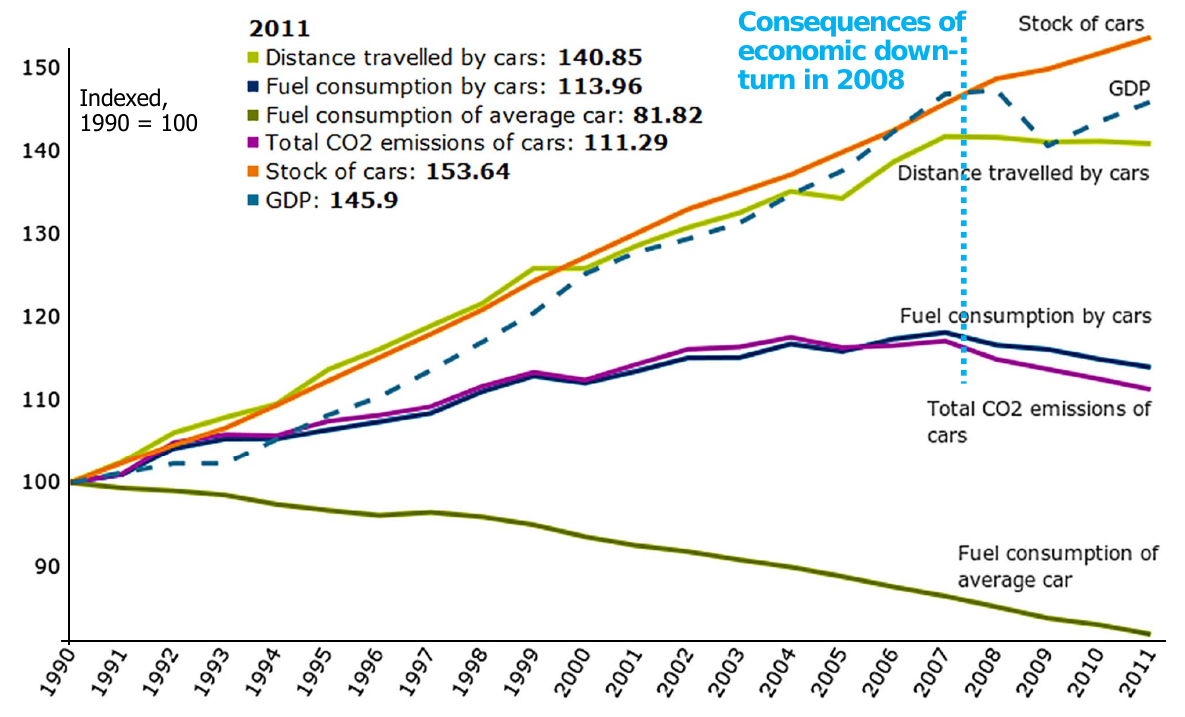
\includegraphics[width=0.85\linewidth]{car_stats}
    \caption{Fuel consumption and \cotwo emissions by cars until 2011}
    \label{fig:car_stats}
\end{figure}

\subsubsection{Household Expenditures}
After the second world war the share of US household income spent on food and energy decreased steadily until 2002.
Lately an increasing share of the household income is spent on energy.
The consumer energy price has been much more volatile than overall consumer prices.
Energy represents $\sim$ 4-5\% of household expenditure.
About half of that (2\%) is electricity.

\subsection{Demand Response (DR)}
The grid requires supply to match demand at all times.
This has traditionally been achieved by letting production follow demand.
Demand response introduces the new paradigm of letting demand follow production.

\subsubsection{Peak Loads}
There is a hierarchy of power generating systems that need to cover for the entire demand, see figure \ref{fig:load_curves}.
Peaks in this demand are very expensive.
This is because these peaks require use of special peaker plants.
These plants are typically gas powered and have low utilization rates.
Generally the faster plants can be ramped up the more expensive they are to use.
Switzerland is in a privileged position because of the large amounts of reservoir hydroplants that can be used to cover for the peak loads.\\

\begin{figure}
    \centering
    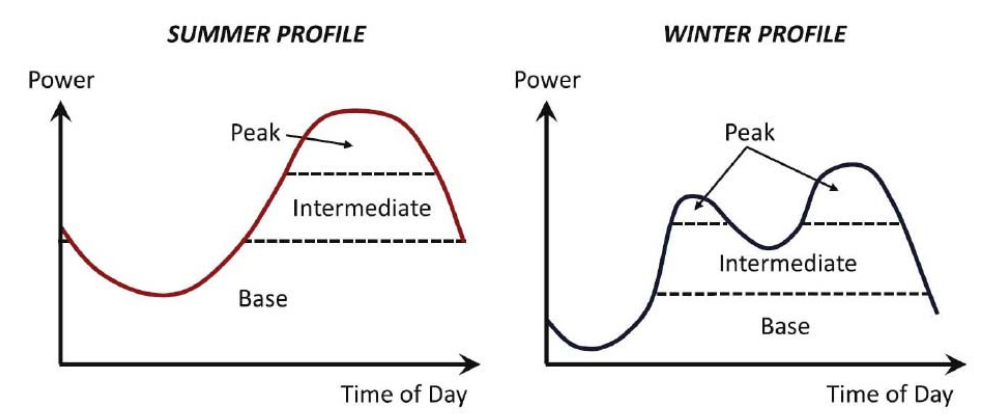
\includegraphics[width=0.7\linewidth]{load_curves}
    \caption{Typical daily load power profiles in the US}
    \label{fig:load_curves}
\end{figure}

The peak demand can be reduced by either load shifting or load shedding, as can be seen in figure \ref{fig:load_shift_shed}.

\begin{figure}
    \centering
    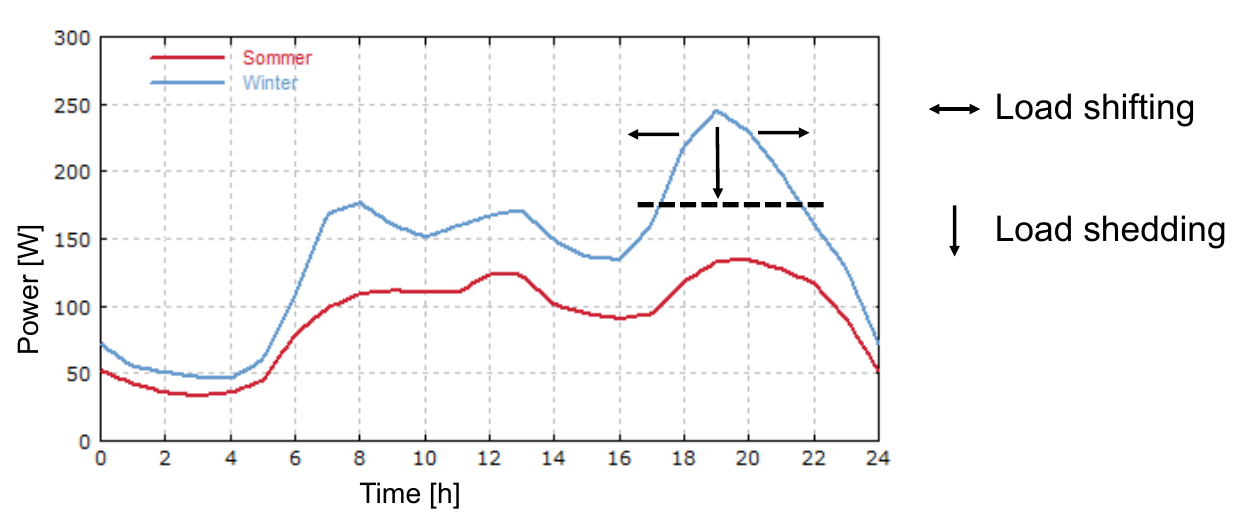
\includegraphics[width=0.8\linewidth]{load_shift_shed}
    \caption{Load shifting and load shedding}
    \label{fig:load_shift_shed}
\end{figure}

\subsubsection{Demand Response for Peak Loads}
Demand response are economical incentives for end-users to change their consumption patterns to reduce peak loads.
Demand response can help in flattening out the load profile and as a response to emergency events.
Demand response can lead to improved grid reliability and lower costs both for utilities and consumers.

\subsubsection{Applying Demand Response}
When a utility company need to decrease the load it send out a demand response signal to any customer being part of a DM program.
The customer then decrease their electricity usage.
These customers have their load measured so that the utility can confirm that the customer does decrease their load.
Customers being part of such a program can be anything from large industrial customers to small residential customers.\\

The special case of demand response for residential customers requires some usefull way of communicating the DM signal.
This can be done through emails, text messages or special hardware.
With integration into home automation system residential DM can also be automated.

\subsubsection{Demand Response Programs}
There are different kinds of demand response programs

\begin{labeling}{\textbf{Critical Peak Pricing (CPP)}}
    \item [\textbf{Time Of Use (TOU)}]
    Fixed rates, not based on current market conditions

    \item [\textbf{Critical Peak Pricing (CPP)}]
    Occasional declaration of a higher price period

    \item [\textbf{Realt Time Pricing (RTP)}]
    Price fluctuation follows market in real time, usually only targeted at industrial customers

\end{labeling}

Figure \ref{fig:dr_programs} shows the relationship between DM programs, control granularity and telemetry.

\begin{figure}
    \centering
    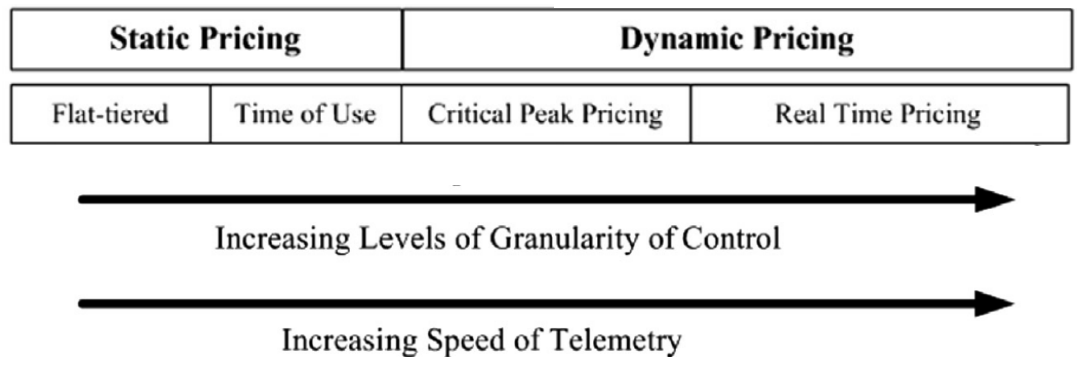
\includegraphics[width=0.7\linewidth]{dr_programs}
    \caption{Demand response programs of increasing control granularity and telemetry speed}
    \label{fig:dr_programs}
\end{figure}

\subsubsection{Consumer Concerns}
Demand response programs face consumer acceptance issues related to
\begin{itemize}
    \item Privacy
    \item External control
    \item Security
    \item Legal issues
\end{itemize}

\subsubsection{Current Use of Demand Response}
In the US demand response is being used to a larger extent than in Europe.
The EU pushes for DR, but there are strong regulatory barriers in most countries.
Switzerland is ahead of the EU, starting field trials of residential DR.

\section{Smart Heating}
Space heating takes up a very large part of the household's energy.
This motivates heating as a prime candidate for applying smart technology.
Space heating is becoming more effective, but the floor area in houses is increasing, making the total energy used for heating stay roughly constant.

\subsection{Factors Impacting Heating}
Factors that impact energy use for heating usually fall in the categories

\begin{itemize}
    \item Building
    \item Heating system
    \item User behavior
    \item Environment
\end{itemize}

\subsection{Thermostats}
Traditional thermostats need to be manually controlled.
The thermostat works as a simple control loop.
Saving energy in this setting would require turning down the heating when leaving home and then coming home to a cold home.
Keeping the temperature lower when away from home saves energy since the heating loss depends on the difference between indoors and outdoors temperatures. \\

\subsubsection{Programmable Thermostats}
Programmable thermostats can keep schedules of different temperatures.
They do require the users to program the schedules to match their daily routine.
Studies have shown that programmable thermostats rarely lead to savings.
Many feel overwhelmed by the programming and simply overrides the features.
Many do not have typical 9-5 jobs, making any programmed schedule unsuitable.

\subsubsection{Self Learning Thermostats}
With self learning thermostats sensors and learning algorithms replace the human in the loop.
The most well known self learning thermostat is the nest.
The nest has a one week intial learning period.\\

Users report a disconnect between their intentions and the heating decisons of self learning thermostats.
Users do not understand why the thermostat takes decisions and feel no way to communicate this to the system.
There is a problem of interpretability, explainability and user experience.

\subsection{Occupancy Sensing and Prediction}
Large savings as well as great comfort could be expected if the heating system knew perfectly where the residents are at all times.
This would require some combination of sensing presence, predicting schedules and adapting to changes in such schedules.

\subsubsection{Occupancy Prediction algorithms}
Prediction is key since heating need to start some time before residents arrive home.
Evaluation of occupancy prediciton algorithms can be done in comparison to a perfect oracle.
The practically achievable best prediction is however worse than any oracle.
The best achievable accuracy is 90\% and many existing algorithms reach an accuracy of 85\%.
Handling of exceptions in these algorithms can be done more or less automatic with sensors or user interaction.

\subsubsection{Conditions Impacting Savings}
Results from studies using occupancy prediction report widely varying energy savings.
Some factors that impact the savings achieved are

\begin{itemize}
    \item Accuracy of prediction
    \item Setback temperature
    \item Power of the heating system
    \item Duration of absence
    \item Building properties (insulation etc.)
    \item Outdoor temperature
\end{itemize}

\subsubsection{Occupancy Sensing}
Sensing occupancy can be done through sensors in the home, such as cameras or motion sensors.
It can also be done using sensors on humans, mainly through reporting of GPS position from a smartphone.
Another possible indicator of occupancy is the electricity consumption.
Extracting an occupancy sequence from electricity consumption data requires use of supervised or unsupervised learning algorithms.
Labeling of such a dataset is difficult for large datasets, making unsupervised or semi-supervised approaches preferable.

\subsection{Estimating Savings Potential of Smart Heating}
In order to simulate heating of buildings one has to create a thermal building model.
This model describes the heat conductivity between the property and environment.
Using such a model one can evaluate which households would achieve substantial savings by using smart heating.
This can then motivate targeting of policy efforts for energy saving.




\section{Non-Intrusive Load Monitoring (NILM)}

\subsection{Load Monitoring}
There exists plenty of smart systems for monitoring the electricity usage of individual appliances.
These often used special plugs that can be difficult to install, expensive and require additional infrastructure.
It would be desirable to be able to get these appliance-individual statistics without special hardware.

\subsubsection{Non-Intrusive Monitoring}
Non-Intrusive Load Monitoring is the idea of only monitoring the aggregated household load with a smart meter and using algorithms to identify consumption of individual devices (disaggregate).
This requires identification of some electric fingerprint for each device.
This is a challenging task, since even devices of the same kind can have bery different electric characteristic (consider for example a new fridge vs an old one that requires defrosting).

\subsubsection{Goals of NILM}
Goals of NILM can be
\begin{itemize}
    \item Detailed consumption feedback
    \item Automatic energy saving recommendations
    \item Occupancy detection for smart heating
\end{itemize}

\subsubsection{Challenges of NILM}
Disaggregating electricity consumption is a challenging task, encountering issues such as

\begin{itemize}
    \item Noise in measurements
    \item Devices with highly variable load
    \item Devices with similair signatures (or even multiple of same device)
\end{itemize}

NILM typically requires a training period during which different devices are switched on and off.
This allows the system to build up a library of electric signatures for different devices.\\

NILM introduces further privacy concerns to smart metering.
Granularity of data and where the data is stored are key issues.

\subsection{Electricity Signatures}
\label{sec:electric_fingerprints}

\subsubsection{Real and Reactive Power}
Capacitive (caused by capacitors) and inductive (caused by inductors) loads change the \textbf{phase shift}, making the current lag behind or lead ahead of the voltage.
From this one can calculate \textbf{real power}
$$
P = I \cdot V
$$
and \textbf{reactive power}
$$
Q = I \cdot V \cdot \sin(\varphi)
$$
where $V$ is voltage, $I$ current and $\varphi$ the phase shift.
Combining mesasurments of real and reactive power creates a 2D-space for electric fingerprints, as can be seen in figure \ref{fig:real_reactive_power}.
Note that even in this 2D space there are still clear clusterings of some appliances.

\begin{figure}
    \centering
    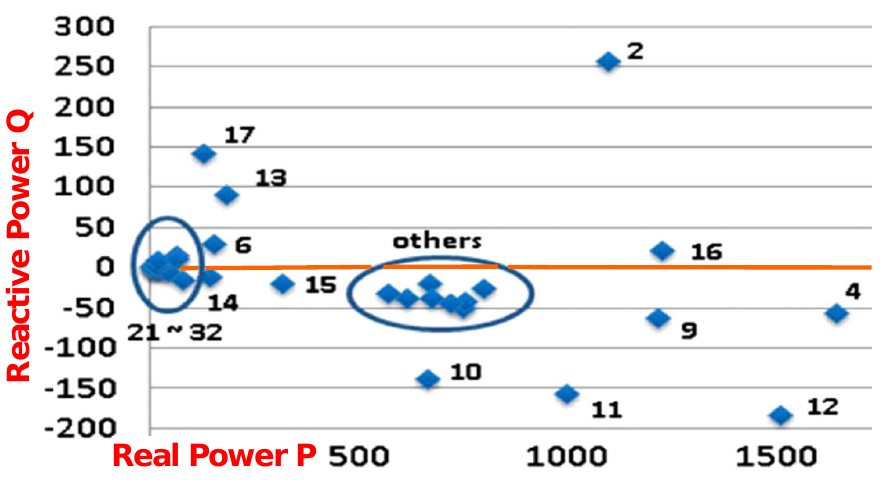
\includegraphics[width=0.70\linewidth]{real_reactive_power}
    \caption{2D-space of electrical fingerprints based on real and reactive power}
    \label{fig:real_reactive_power}
\end{figure}

\subsubsection{Voltage-Current Trajectories}
One way to create a more detailed electric fingerprint is to also consider the dimension of time.
Some appliances (for examples appliances containing motors) have very specific shapes of voltage and current curves.
This motivates using a voltage-current trajectory, see figure \ref{fig:voltage_current_trajectories}, as fingerprint.
Note that measuring these trajectories requires rather high efforts.

\begin{figure}
    \centering
    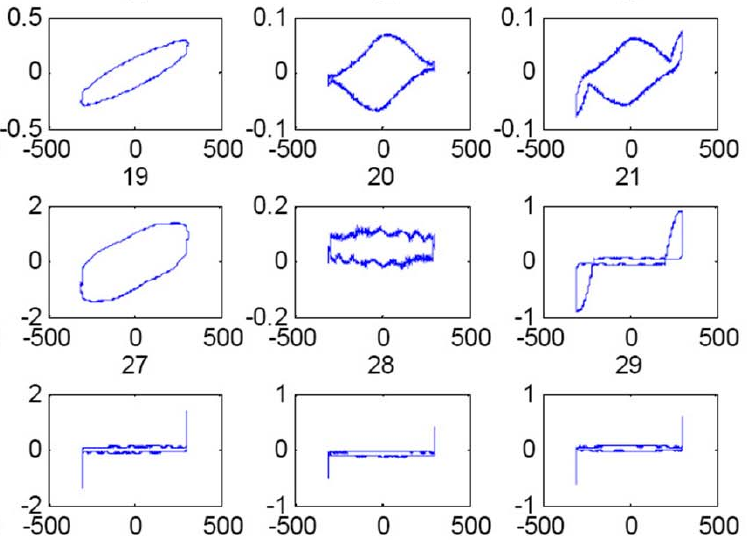
\includegraphics[width=0.60\linewidth]{voltage_current_trajectories}
    \caption{Examples of voltage-current trajectories}
    \label{fig:voltage_current_trajectories}
\end{figure}

\subsubsection{Higher Resolution Load Signatures}
If measurements are performed at $\gg 50$ Hz the shape of the current or power waveform itself can be used as a fingerprint.
Examples can be seen in \ref{fig:nilm_waveform}.
With high enough sampling frequency one can even consider the shape of single turn-on and turn-off events for different appliances.
Signatures can also be used from freqency analysis.
Another frequency-based signature is the Electromagnetic Interfernece (EMI) of different devices.
Note however that frequency measurements require very high sampling rates (As per the sampling theorem one has to sample with twice the frequency of the highest frequency component of interest).

\begin{figure}
    \centering
    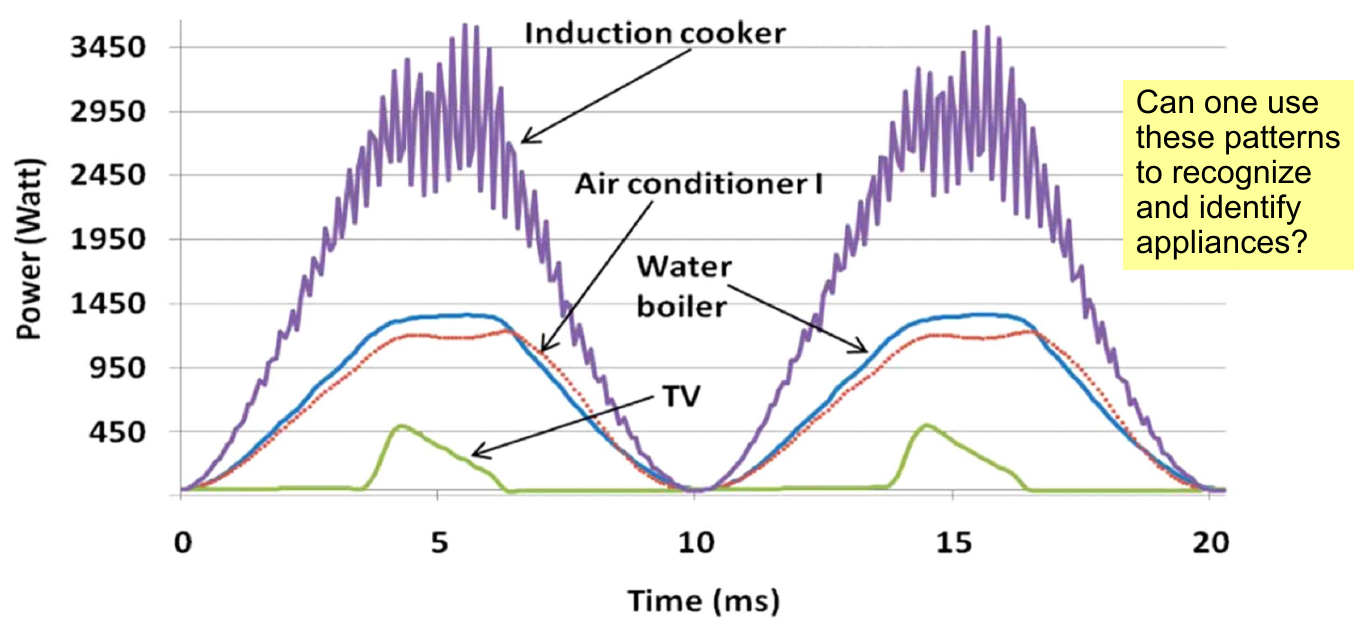
\includegraphics[width=0.70\linewidth]{nilm_waveform}
    \caption{Examples of power waveform as electric fingerprint}
    \label{fig:nilm_waveform}
\end{figure}

\subsection{Building a Signature Database}
A complete database of electric signatures can combine any of the fingerprints in \ref{sec:electric_fingerprints}.
It can include both signatures of on-off switches and of running appliances.
Building this database requires a learning phase.
Learning can be done completelty manually (recording switching on and off appliances) or by learning them automatically (supervised or unsupervised training).
Some generic features could be retrieved from global databases to simplify learning.\\

\subsection{The NILM process}
The complete NILM process generally look like

\begin{enumerate}
    \item Capture data
    \item Normalize adn filter out noise
    \item Detect events
    \item Match signature to database
    \item Application specific processing
\end{enumerate}


\section{Smart Grid Security}
Electricity is a key resource and therefore the grid is part of critical infrastructure.
Energy security typically has referred to geopolitics, accidents and natural disasters.
Energy security is increasingly a matter of cyber security.

\subsection{Critical Infrastructure}
Critical infrastructure is infrastructure that is a critical enabler of economic activity and social welfare.
Economies tend to become increasingly specialized and rely more on critical infastructure for key resources and services.\\

The electrical grid has evolved over a long time and therefore contains of a mix of old and new technology.
The electrical grid is a patchwork of both physical and organizational networks.
It is highly dynamic and mutually interdependent with other critical infrastructure (in particular ICT).
This creates risk for cascading effects if one piece of critical infrastructure should break down.
Cyber attacks against critical infrastructure has been proven to be a real threat.

\subsection{Fragility of Electricity Grids}
The implementation of smart grids potentially increase reliability thanks to fault detection and isolation.
Islanding (isolating self sustaining portions of the grid from problems) can make the grid more robust.
These improvements do however come at a cost of increased complexity and a larger attack surface for cyber attacks.\\

The physcial properties of electricity make the grid particularly hard to control.
Electricity travels at the speed of light, making it impossible for human decisionmakers to react to problems.
Electricity flows in all paths available and can not easily be stopped with some valve or switch.\\

\begin{tcolorbox}
    \textbf{Blackouts}
    \begin{labeling}{\textbf{Germany, 2006}}
    \item [\textbf{US, 2003}]
        A tree flashover caused a domino effect.
        Operators did not notice that power lines went out of service because of bug (race condition) in monitoring software.
    \item [\textbf{Italy, 2003}]
        Tree flashover in Switzerland caused blackout of nearly all of Italy through domino effect.
    \item [\textbf{Germany, 2006}]
    Scheduled shutdown of a line to allow a crusie ship safe passage results in unforseen cascade of line overloads.
        Europe was split in separate areas to stop cascade.
        Luckily automatic countermeasures managed to rebalance the grid.
    \end{labeling}

Blackouts of the electrical grids in all cases spilled over and severly crippled other critical infrastructure.
All these failures show that local problems quickly result in far-reaching consequences.
\end{tcolorbox}

\subsection{Cyber Attacks Against the Electrical grid}
The smart grid presents large challenges in cyber security.
The industry trend is to replace specialized software and hardware with commercial off-the-shelf systems using general internet based technology.
Physical security is an issue, especially considering the locations of much of the smart grid technology.
Maintaining high security as grids are getting smarter proves to be a challenge since most utilities do not have much experience with cyber security.\\

Some properties and changes of the smart grid that increases the attack surface are
\begin{itemize}
    \item Legacy systems
    \item Increased interconnection of systems
    \item New 2-way systems
    \item New customer touch points
    \item More subsystems, larger code base
\end{itemize}

\subsubsection{Examples of Cyber Attacks Against Electricity Infrastructure}
\begin{labeling}{\textbf{SQL Slammer Worm}}
    \item [\textbf{SQL Slammer Worm}]
    Worm that infected US nuclear power plant in 2003.
    Spread through business network to control network, eventually causing a denial of service of the control system.
    Fortunately did not affect analog backup system.
    \item [\textbf{Stuxnet}]
    Highly specialized computer worm infecting Windows systems. Carries malware payload specifically targeted at Siemens control systems.
    The target of Stuxnet was the Iranian uranium enrichment infrastructure.
    It is largely believed that the worm was created by US and Israelian cyber warfare institutions.
\end{labeling}

\section{ICT Abatement Potential and Rebound Effects}

\subsection{Abatement through ICT}

\begin{table}[h]
    \begin{tabular}{| c | l | l | l |}
    \hline
    \textbf{Sector} & \textbf{\makecell[l]{Substitution, \\ Dematerialization}} & \textbf{Increased Efficiency} & \textbf{\makecell[l]{Awareness and \\ decision support}} \\ \hline
    Transportation &
    \makecell[l]{Telepresence,\\Telework,\\Virtual conferences} &
    \makecell[l]{Route optimization} &
    \makecell[l]{Mobility footprint \\monitoring, \\Real time navigation}\\ \hline
    Households &
    E-shopping &
    Smart heating &
    \makecell[l]{In-home displayes,\\Normative feedback} \\ \hline
    Industry &
    \makecell[l]{3D printing,\\Virtual goods} &
    \makecell[l]{Smart heating,\\Smart logistics,\\Robots,\\AI-based automation} &
    \makecell[l]{Integrated supply chain} \\ \hline
    Energy &
    (Renewable integration) &
    \makecell[l]{Automatic demand \\response} &
    \makecell[l]{User based \\demand response,\\Gas leakage discovery} \\ \hline
    \end{tabular}

    \caption{Abatement potential of ICT in different sectors}
\end{table}

\subsection{The Rebound Effect}
The typical process of the rebound effect is as follows

\begin{enumerate}
    \item Baseline consumption
    \item Efficiency increase
    \item Product is more efficient, but also cheaper
    \item Increased consumption
\end{enumerate}

\begin{tcolorbox}
    \textbf{A Neoclassical Economics Perspective}\\

        \begin{center}
        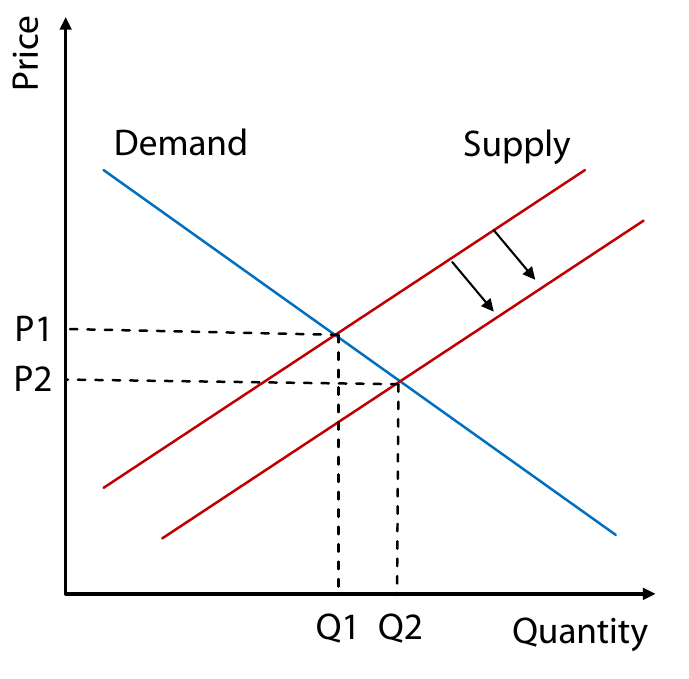
\includegraphics[width=0.50\linewidth]{rebound_market}
        \captionof{figure}{Market equilbrium before and after efficiency increase}\
        \label{fig:rebound_market}
        \end{center}

    Figure \ref{fig:rebound_market} shows the relationship between price, quantity, demand and supply.
    The market equilibrium maximizes the output.
    As efficiency increases, the producer's costs decreases.
    This pushes the supply curve down and a new equilibrium is reached.
    In this new equilibrium the prize is lower and the output higher.
\end{tcolorbox}

\subsubsection{Direct Rebound Effect}
Direct rebound is the counterbalance of the same good for which efficiency increased.
The direct rebound is typically expressed as a percentage.
An example from the transport sector is cars getting more efficient, leading to lower running costs and therefore people drive further and more often.

\subsubsection{Indirect Rebound Effect}
People do not spend their income on just one good, but rather on a whole set of goods.
Efficiency increase of one and the following price decrease rebalances what can be spent on different goods.
One good getting cheaper can thereby result in increased consumption of some other good.
Consider for example again the case of more efficient cars.
Instead of simply driving more the money saved could be used to travel more, paying for more flights.

\subsubsection{Limits of Rebound Effect}
Not all goods are affected by rebound effects.
Consider goods where a lower price does not particularly increase consumption (for example vacuum cleaners).
Also in cases where the energy is a minor cost component an increased energy efficiency doesn't affect the price much and therefore no rebound effect is observed.
It is also worth considering that not all increased consumption is negative.
For example increased use of train rides substituting some car rides would be beneficial from a sustainability viewpoint.\\

\begin{tcolorbox}
    \textbf{The Kaya Identity}\\
    The following relationship describes factors that affect \cotwo emissions.\\

    \begin{tabular}{ccccccccc}
        Emissions &
        $=$ &
        Population &
        $\cdot$ &
        Affluence &
        $\cdot$ &
        Energy Intensity &
        $\cdot$ &
        Carbon Intensity
        \\
        $\frac{\text{Gt\cotwo}}{year}$ & &
        Persons & &
        $\frac{\text{\$} / \text{person}}{\text{year}}$ & &
        $\frac{\text{kWh}}{\text{\$}} $ & &
        $\frac{\text{Gt\cotwo}}{\text{kWh}}$
    \end{tabular}

    \begin{itemize}
        \item Population will grow.
        \item De-growth proponements aim at limiting affluence.
        \item ICT can mainly contribute to decreasing energy intensity.
        \item ICT also has a central role in transition to zero carbon technology to decrease carbon intesity.
        \item In the EU the carbon intensity is decreasing.
    \end{itemize}
\end{tcolorbox}





\section{The Energy Consumption of ICT}
Since the early days of computing the energy conspumption of ICT has been discussed.
It is generally a topic with little consensus and widely varying estimates of emissions  attributed to computing.

\subsection{Network Technology}
Computer networks can be divided into multiple stages between the backbone of the internet and consumer devices.
Close to the consumers in the networks are Digital Subscriber Line Access Multiplexers (DSLAMs).
These are local nodes providing neighborhoods with internet connection.
In the backbone of the network are poweful core internet routers.
Network-related devices are typically split into the three categories: User, Network and Data centre.

\subsection{Data Centers (DCs)}
Data centers are typically located in cold areas, often with supply to water closeby.
Large data centers have their own energy supply stations.

\subsubsection{PUE}
The Power Usage Efficiency (PUE) is a measure of efficiency of a data center.
It can be calculated as
$$
\text{PUE} = \frac{\text{Energy consumption of entire DC}}{\text{Energy for IT equipment}}
= 1 + \frac{\text{Non-IT energy}}{\text{IT Energy}}
$$
The non-IT energy consist mainly of cooling.
Some energy is spent on lighting and some is lost in transformation.
The average PUE values improved substantially until 2011.
The biggest infrastrucutre efficiency gains happened 5 years ago.
Further improvements require significant investments.
Google report PUEs as low as 1.12.

\subsubsection{Cooling}
Data centers are generally air cooled through a Computer Room Air Conditioning Unit (CRAC).
DCs are usually built with a raised floor to allow pumping of cold air under the floor.
A more modern layout is alternating cold and hot aisles between servers.
Some alternative concepts that are still in the research stage are server immersion cooling and on-chip water cooling.
Efforts exist to reuse heat from DCs in district heating.

\subsubsection{Servers in the World}
About half of servers are in data centers.
The other half are directly at enterprises.
Servers can be estimated responsible for 200-300 TWh/year.
This represents less than 2\% of worldwide electricity consumption.

\subsection{The Network}
The network can be modelled top down (start by estimating equipment) or bottom up (start by estimating users and usage).
Top down models tend to overstate consumption whereas bottom up models tend to understate consumption.
It is often somewhat unclear what equipment should be considered part of the internet.\\

Energy intensity of equipment close to customers is usually more time dependent.
Energy intensity of equipment deeper in the network depends more on traffic.

\subsubsection{Network Growth}
The data sent over the internet has grown rapidly and continues to do so.
In particular global mobile traffic and machine-to-machine traffic is growing with high rates.
The energy required by data centers is estimated to increase substantially in order to handle this increased traffic.
The increase in energy efficiency is lower than the growth of traffic.

\subsection{Future Predictions}
The overall wroldwide electricity consumption of PCs has increased.
The growth has been (and continues to be) driven by

\begin{itemize}
    \item Higher penetration rates
    \item Increased hours of use
    \item More powerful PCs
    \item Larger screens
\end{itemize}

In households in mature markets low-power devices such as tablets and smartphones are substituting PCs and laptops.
For these low-power devices a larger fraction of their environmental impact comes from production (instead of use).
Functional convergence also decreases the amount of devices needed.


\section{Electrical Vehicles}

\subsection{Transportation}
A third of the total energy use of the EU goes into transport.
Road transport is the main reason behind emissions.
Transport has been increasing and continues to increase.
In the US and Europe petroleum is the main energy source for transportation.\\

Measuring the efficiency can be done in multiple ways.

\begin{itemize}
    \item Energy consumption / distance traveled
    \item Emissions / distance traveled
    \item Emissions / person-kilometer (pkm)
    \item Emissions / ton and km (for cargo)
\end{itemize}

\subsection{Motivation behind Electrical Vehicles (EVs)}
The demand for cars is increasing and expected to triple in the next 30 years.
The main growth is in developing countries.
On the other hand the oil supply is very limited and expected to decline.
This does not add up and major changes in the car industry are likely.
Many countries have set ambitious goals for the development of EVs.

\subsubsection{Regenerative Breaking}
When slowing down in traffic kinetic energy is wasted.
By regenerative breaking an electric engine can be used as a generator and recover some of breaking energy.
Regenerative breaking typically only requires a small engine and battery.

\subsection{Current state of EV fleet}
In most countries electrical vehicles and hybrids represent a tiny part of the countries car fleet.
Registrations of EVs are however increasing.
An exception is Norway, where EVs and hybrids represent 51\% of new car sales.
This early adoption can be attributed to strong political incentives providing financial subsidies for EVs.

\subsection{Challenges}

\begin{labeling}{\textbf{Battery conflicts}}
    \item [\textbf{Cost}]
    The main cost of EVs has been batteries.
    Battery costs are however currently coming down quickly.
    \item [\textbf{Battery safety}]
    The combination of high energy and flammable materials make battery pack safety an important concern.
    A number of safety tests have to be passed before batteries are certified safe.
    \item [\textbf{Battery lifetime}]
    We typically expect to use cars for a much longer timespan than other battery powered devices.
    \item [\textbf{Battery conflicts}]
    Requirements on battery power, lifetime, recharge time and cost often conflict.
    Battery technology that handles these conflicts exists, but is still expensive.
    The most commonly used type today is Li-ion.
    \item [\textbf{Driving range}]
    The driving range of EVs has increased a lot in the last years.
    In reality the vast majority of trips are very short.
    Statistically almost all trips can be covered by the driving range of modern EVs.
\end{labeling}

\subsection{Types of EVs}
Electrical vehicles can be split into three groups.

\subsubsection{Battery Electric Vehicles (BEV)}
BEVs are only electric and therefore have a comparably limited driving range. They take multiple hours to charge.

\subsubsection{Plug-in hybrid EV (PHEV)}
PHEVs use regenerative breaking as well as plug charging.
They reach higher driving ranges as they can utilize the gasoline engine.
The battery is typicaly smaller than in BEVs and charging thereby faster.

\subsubsection{Hybrid Electric Vehicle (HEV)}
HEVs are only equipped with regenerative braking.
They are generally similar to gasoline-powered cars.\\

PHEVs and HEVs can act as a bridging technology for a transition to EVs.
These types of EVs relieve any range anxiety of consumers.
More people using hybrids creates motivation for investing in network of charging places.
This in turn make more people consider BEVs as a viable option.

\subsection{Effect of EVs on the Grid}
Replacement of all cars with EVs would nearly double the electricity consumption of households.
This creates a major concern for the grid.
EV charging can be considered in multiple ways

\begin{itemize}
    \item Home charging
    \item Public charging
    \item Semi-public charging (e.g. at work)
    \item Special operation centers
\end{itemize}

If all EVs are charged at home this would create massive peaks as people come home from work in the evening.
Similar effects could be expected if everyone charged at work, since most people arrive to work at similar times.
Load management that spreads out the charging over time can help relieve these issues somewhat.
Even with load management cars moving in clusters between the city during the day and suburbs during the evening can be a challenge for the grid.





\end{document}

